\documentclass{article}
\usepackage{graphicx, amsmath}
\graphicspath{ {./images/} }

\title{HW 7.4 Solns}
\author{Principles of Microeconomics}
\date{\today}

\begin{document}

\maketitle

\subsection*{Ch. 7 \#9, 10}

\begin{enumerate}
\setcounter{enumi}{8}

\item

	\begin{enumerate}
	
	\item The advancement in production technology will shift the supply curve out. That increases the equilibrium quantity and decreases the equilibrium price. As a result, consumer surplus and producer surplus both increase.
	
		\begin{center}
		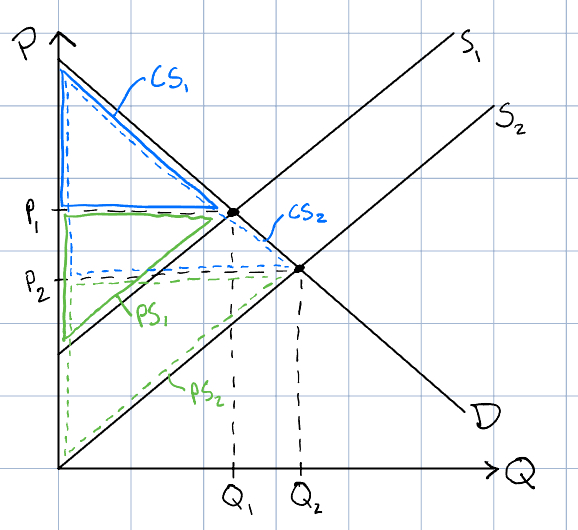
\includegraphics[width = 0.5\textwidth]{paa9a}
		\end{center}
	
	\item That makes typewriters and computers substitutes. The decreased price of computers shifted demand for typewriters left. That decreases the equilibrium quantity and price. As a result, consumer surplus and producer surplus both decrease. Typewriter producers should be sad about the technological advance because it decreases the value they accrue in the typewriter market.
	
	\begin{center}
	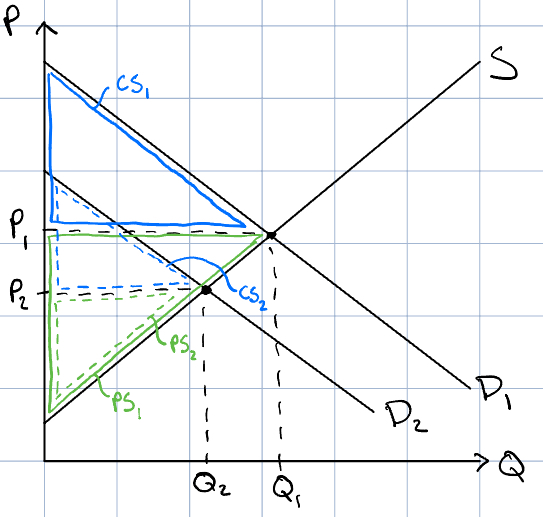
\includegraphics[width = 0.5\textwidth]{paa9b}
	\end{center}
	
	\item Computers and software are complements, so the decreased price of computers increases demand for software. That increases the equilibrium quantity and price of software. As a result, consumer surplus and producer surplus both increase. Software producers should be happy about the technological advance because it increases the value they accrue in the software market.
	
	\begin{center}
	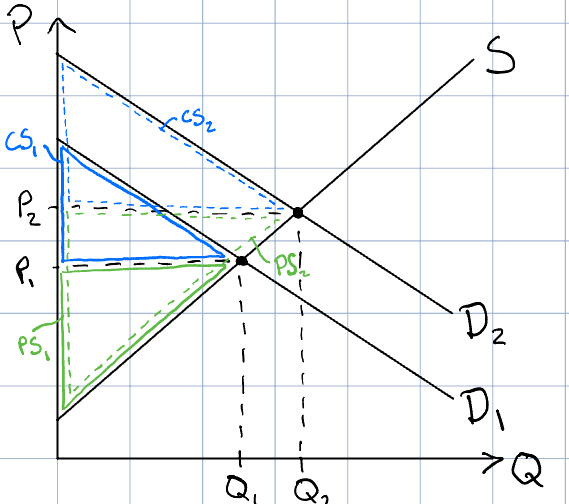
\includegraphics[width = 0.5\textwidth]{paa9c}
	\end{center} 
	
	\item It does. We see that software producers accrued a lot more surplus when computers became more widespread.
	
	\end{enumerate}
	
\item

	\begin{enumerate}
	
	\item Provider A: \$0 because each additional movie comes at no additional charge. \\
		Provider B: \$1 because each additional movie comes at a charge of \$1.
		
	\newpage	
	
	\item The friend should buy until their willingness to pay for an additional movie equals the cost of an additional movie. \\
		
		\begin{center}
		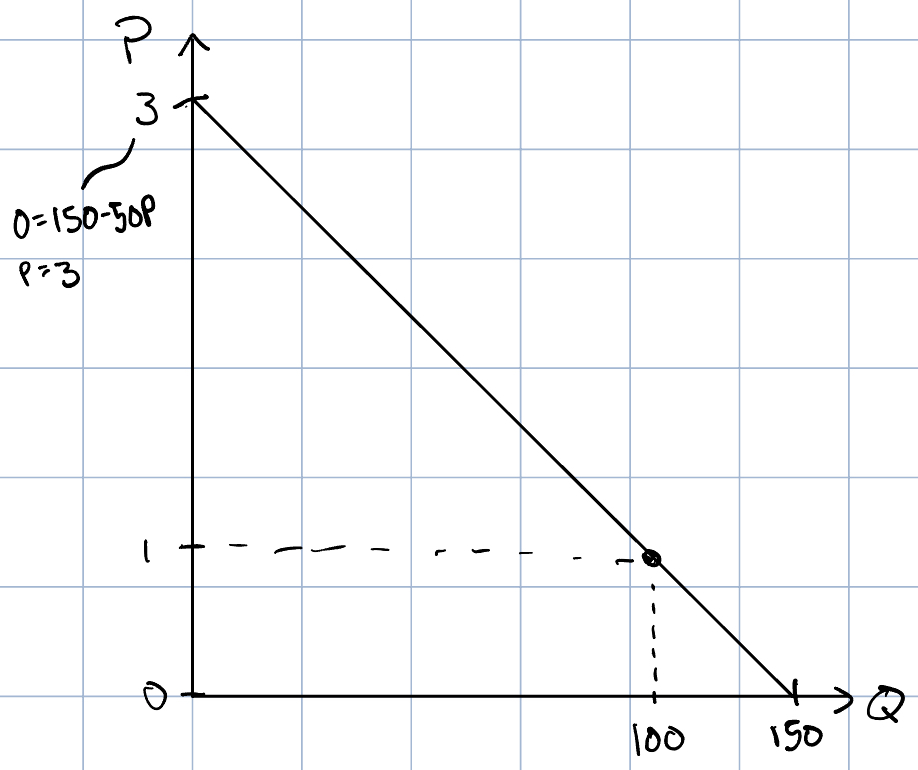
\includegraphics[width = 0.5\textwidth]{paa10}
		\end{center}
		
		Provider A: $Q_D = 150 - 50(0) = 150$\\ 
		Provider B: $Q_D = 150 - 50(1) = 100$
	
	\item She would pay Provider A the one time flat fee of \$120. She would pay Provider B \$1 per move, \$100.
	
	\item Provider A: (We have to think about price a little differently here) \\
		Value accrued from movies = $\frac{1}{2}(3)(150) = 225$ \\
		Total spent on movies = \$120 \\
		Consumer Surplus = $225 - 120 = \$105$ \\
		Provider B: \\
		Consumer Surplus = $\frac{1}{2}(3 - 1)(100) = \$100$
	
	\item I would recommend Provider A because they would get more consumer surplus from streaming through Provider A.
	
	\end{enumerate}

\end{enumerate}

\subsection*{Non-Mankiw \#1, 2}

\end{document}